%\documentclass[professionalfonts,10pt]{beamer}
\documentclass[professionalfonts,10pt,handout]{beamer}

\usepackage[T1]{fontenc}
\usepackage[utf8]{inputenc}
\usepackage[english]{babel}
\usepackage{pgfplots}
\pgfplotsset{compat=1.9}
\usepackage{booktabs}
\usepackage{siunitx}
\usepackage{bbding}
\usepackage{cmbright}
\usepackage{helvet}
\usepackage{multirow}
\usepackage{tikz}

\usetikzlibrary{shapes.callouts,shapes.geometric,arrows}
\tikzstyle{stazione} = [circle,thick,draw=black!40,fill=black!30,text=white,minimum size=0.9cm,font=\bfseries]
\tikzstyle{nodobianco} = [rectangle,rounded corners,minimum width=1.0cm,minimum height=0.5cm,text centered,draw=white,fill=black!40,text=white]
\tikzstyle{nododummy} = [rectangle,rounded corners,minimum width=1.0cm,minimum height=0.5cm,text centered,draw=white,fill=white,text=black]
\tikzstyle{eventoblue} = [circle,thick,draw=blue,fill=white,minimum size=0.1cm]
\tikzstyle{eventomarrone} = [circle,thick,draw=brown,fill=white,minimum size=0.1cm]
\tikzstyle{eventorosso} = [circle,thick,draw=red,fill=white,minimum size=0.1cm]
\tikzstyle{eventonero} = [circle,thick,draw=black,fill=white,minimum size=0.1cm]
\tikzstyle{phase} = [rectangle,rounded corners,minimum width=2cm,minimum height=0.4cm,text centered,draw=black,fill=red!10]
\tikzstyle{io} = [trapezium,trapezium left angle=80,trapezium right angle=100,minimum width=1cm,minimum height=0.4cm,text centered,draw=black,fill=blue!10]
\tikzstyle{process} = [rectangle,rounded corners,minimum width=2cm,minimum height=0.4cm,text centered,draw=black,fill=green!10]
\tikzstyle{comment} = [rectangle,rounded corners,minimum width=0.1cm,minimum height=0.1cm,text centered,draw=white,fill=white,text=red]
%\tikzstyle{io} = [trapezium, trapezium left angle=70, trapezium right angle=110, minimum width=2cm, minimum height=0.5cm, text centered, draw=black, fill=blue!30]
%\tikzstyle{process} = [rectangle, minimum width=3cm, minimum height=1cm, text centered, draw=black, fill=orange!30]
%\tikzstyle{decision} = [diamond, minimum width=3cm, minimum height=1cm, text centered, draw=black, fill=green!30]
\tikzstyle{arrow} = [thick,->,>=stealth]

\usepackage{datetime}
\newdate{date}{18}{02}{2015}

%\usetheme[department=management,showsection=true]{DTU}

\newcommand{\st}{\text{s.t.}}
\newcommand{\tc}{\, : \,}
\newcommand{\ov}[1]{\overline{#1}}
\newcommand{\un}[1]{\underline{#1}}
\newcommand{\gb}[1]{\boldsymbol{#1}}


	
\newcommand{\tabitem}{{\color{dtured}$\bullet$} }

\begin{document}


%\frame{
%\frametitle{Students Evaluation}
%\input{../students.tex}
%}






\frame{
\frametitle{Example of Space-Time Graph: Train A}

\begin{columns}
\begin{column}{0.4\textwidth}
\vspace{-0.8cm}
\begin{table}
\begin{scriptsize}
\setlength{\tabcolsep}{4.5pt}
\renewcommand{\arraystretch}{1.2}
\begin{center}
\begin{tabular}{lrrr}
\multicolumn{4}{c}{\bf \colorbox{black}{\bfseries\textcolor{white}{Ideal Profits and Shift/Stretch Penalties}}} \\
\toprule
 & \bf \textcolor{blue}{Train A} & \bf \textcolor{red}{Train B} & \bf \textcolor{brown}{Train C} \\
\cmidrule(lr){2-2} \cmidrule(lr){3-3} \cmidrule(lr){4-4}
Ideal profit $pr_j$          & 4 & 5 & 3 \\
Shift penalty $\pi_j^{sh}$   & 1 & 1 & 1 \\
Stretch penalty $\pi_j^{st}$ & - & 1 & - \\
\bottomrule
\end{tabular}
\end{center}
\end{scriptsize}
\end{table}
\end{column}
\begin{column}{0.6\textwidth}
\begin{table}
\begin{scriptsize}
\setlength{\tabcolsep}{3pt}
\renewcommand{\arraystretch}{1.2}
\begin{center}
\begin{tabular}{lrrrrrr}
\multicolumn{7}{c}{\bf \colorbox{black}{\bfseries\textcolor{white}{Ideal Timetables}}} \\
\toprule
 & \multicolumn{2}{c}{\bf \textcolor{blue}{Train A}} & \multicolumn{2}{c}{\bf \textcolor{red}{Train B}} & \multicolumn{2}{c}{\bf \textcolor{brown}{Train C}} \\
\cmidrule(lr){2-3} \cmidrule(lr){4-5} \cmidrule(lr){6-7}
\bf Station & \bf Arr & \bf Dep & \bf Arr & \bf Dep & \bf Arr & \bf Dep \\
\cmidrule(lr){1-7}
1       &      & 9:10 &      & 9:05 &      &      \\
2       & 9:15 &      & 9:09 & 9:11 &      & 9:08 \\
3       &      &      & 9:15 &      & 9:13 &      \\
\bottomrule
\end{tabular}
\end{center}
\end{scriptsize}
\end{table}
\end{column}
\end{columns}
\vspace{-0.5cm}
\begin{center}
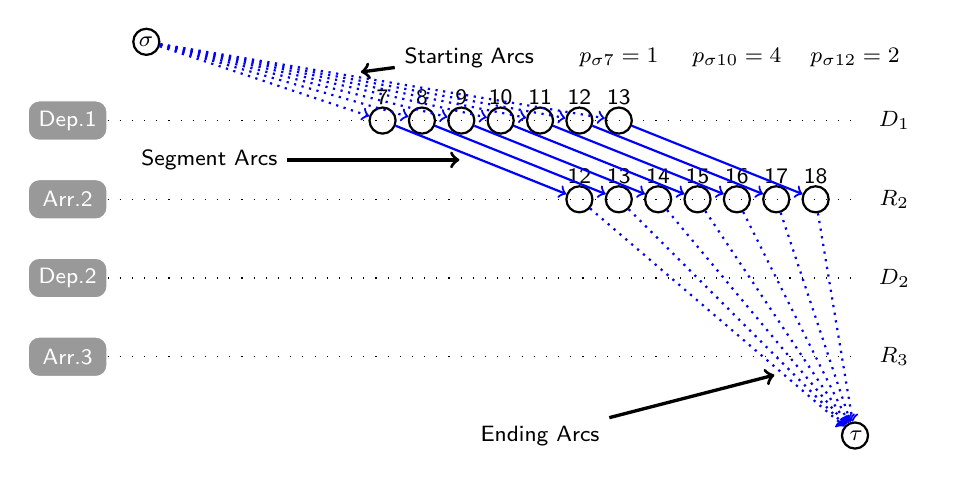
\begin{tikzpicture}
\tikzstyle{every node}=[font=\sffamily\footnotesize]

% minute = 0.5cm

\node (aaa) [xshift=5.5cm,yshift=0.8cm] {$p_{\sigma 7} = 1$};
\node (bbb) [right of=aaa,xshift=0.5cm] {$p_{\sigma 10} = 4$};
\node (ccc) [right of=bbb,xshift=0.5cm] {$p_{\sigma 12} = 2$};

\node (lbl1) [xshift=3.6cm,yshift=0.8cm] {Starting Arcs};
\node (lbl1e) [left of=lbl1,xshift=-0.5cm,yshift=-0.2cm] {};

\node (lbl2) [xshift=0.3cm,yshift=-0.5cm] {Segment Arcs};
\node (lbl2e) [right of=lbl2,xshift=2.3cm,yshift=0cm] {};

\node (lbl4) [xshift=4.5cm,yshift=-4.0cm] {Ending Arcs};
\node (lbl4e) [right of=lbl4,xshift=2.1cm,yshift=0.8cm] {};

\node (1D)  [nodobianco,xshift=-1.5cm] {Dep.1};
\node (2A)  [nodobianco,below of=1D] {Arr.2};
\node (2D)  [nodobianco,below of=2A,yshift=0.0cm] {Dep.2};
\node (3A)  [nodobianco,below of=2D] {Arr.3};

\node (1De)  [nododummy,right of=1D,xshift=9.5cm] {$D_1$};
\node (2Ae)  [nododummy,right of=2A,xshift=9.5cm] {$R_2$};
\node (2De)  [nododummy,right of=2D,xshift=9.5cm] {$D_2$};
\node (3Ae)  [nododummy,right of=3A,xshift=9.5cm] {$R_3$};

\node (sigma)[eventonero,label={[label distance=-0.4cm]0:{$\sigma$}},above of=1D,xshift=1cm,yshift=0cm] {};
\node (tau)  [eventonero,label={[label distance=-0.4cm]180:{$\tau$}},below of=3A,xshift=10cm,yshift=0cm] {};

\node (D107)[eventonero,label={[label distance=-0.1cm]90:{7}},right of=1D,xshift=3.0cm,yshift=0cm] {};
\node (D108)[eventonero,label={[label distance=-0.1cm]90:{8}},right of=D107,xshift=-0.5cm,yshift=0cm] {};
\node (D109)[eventonero,label={[label distance=-0.1cm]90:{9}},right of=D108,xshift=-0.5cm,yshift=0cm] {};
\node (D110)[eventonero,label={[label distance=-0.1cm]90:{10}},right of=D109,xshift=-0.5cm,yshift=0cm] {};
\node (D111)[eventonero,label={[label distance=-0.1cm]90:{11}},right of=D110,xshift=-0.5cm,yshift=0cm] {};
\node (D112)[eventonero,label={[label distance=-0.1cm]90:{12}},right of=D111,xshift=-0.5cm,yshift=0cm] {};
\node (D113)[eventonero,label={[label distance=-0.1cm]90:{13}},right of=D112,xshift=-0.5cm,yshift=0cm] {};

\node (A212)[eventonero,label={[label distance=-0.1cm]90:{12}},right of=2A,xshift=5.5cm,yshift=0cm] {};
\node (A213)[eventonero,label={[label distance=-0.1cm]90:{13}},right of=A212,xshift=-0.5cm,yshift=0cm] {};
\node (A214)[eventonero,label={[label distance=-0.1cm]90:{14}},right of=A213,xshift=-0.5cm,yshift=0cm] {};
\node (A215)[eventonero,label={[label distance=-0.1cm]90:{15}},right of=A214,xshift=-0.5cm,yshift=0cm] {};
\node (A216)[eventonero,label={[label distance=-0.1cm]90:{16}},right of=A215,xshift=-0.5cm,yshift=0cm] {};
\node (A217)[eventonero,label={[label distance=-0.1cm]90:{17}},right of=A216,xshift=-0.5cm,yshift=0cm] {};
\node (A218)[eventonero,label={[label distance=-0.1cm]90:{18}},right of=A217,xshift=-0.5cm,yshift=0cm] {};

%\draw[dotted] or \draw[densely dotted] or \draw[loosely dotted]

\draw[very thick,->] (lbl1) -- (lbl1e);
\draw[very thick,->] (lbl2) -- (lbl2e);
\draw[very thick,->] (lbl4) -- (lbl4e);

\draw[loosely dotted] (1D) -- (1De);
\draw[loosely dotted] (2A) -- (2Ae);
\draw[loosely dotted] (2D) -- (2De);
\draw[loosely dotted] (3A) -- (3Ae);

\draw[blue,thick,dotted,->] (sigma) -- (D107);
\draw[blue,thick,dotted,->] (sigma) -- (D108);
\draw[blue,thick,dotted,->] (sigma) -- (D109);
\draw[blue,thick,dotted,->] (sigma) -- (D110);
\draw[blue,thick,dotted,->] (sigma) -- (D111);
\draw[blue,thick,dotted,->] (sigma) -- (D112);
\draw[blue,thick,dotted,->] (sigma) -- (D113);
\draw[blue,thick,->] (D107) -- (A212);
\draw[blue,thick,->] (D108) -- (A213);
\draw[blue,thick,->] (D109) -- (A214);
\draw[blue,thick,->] (D110) -- (A215);
\draw[blue,thick,->] (D111) -- (A216);
\draw[blue,thick,->] (D112) -- (A217);
\draw[blue,thick,->] (D113) -- (A218);
\draw[blue,thick,dotted,->] (A212) -- (tau);
\draw[blue,thick,dotted,->] (A213) -- (tau);
\draw[blue,thick,dotted,->] (A214) -- (tau);
\draw[blue,thick,dotted,->] (A215) -- (tau);
\draw[blue,thick,dotted,->] (A216) -- (tau);
\draw[blue,thick,dotted,->] (A217) -- (tau);
\draw[blue,thick,dotted,->] (A218) -- (tau);

\end{tikzpicture}
\end{center}
}





\frame{
\frametitle{Example of Space-Time Graph: Train B}

\begin{columns}
\begin{column}{0.4\textwidth}
\vspace{-0.8cm}
\begin{table}
\begin{scriptsize}
\setlength{\tabcolsep}{4.5pt}
\renewcommand{\arraystretch}{1.2}
\begin{center}
\begin{tabular}{lrrr}
\multicolumn{4}{c}{\bf \colorbox{black}{\bfseries\textcolor{white}{Ideal Profits and Shift/Stretch Penalties}}} \\
\toprule
 & \bf \textcolor{blue}{Train A} & \bf \textcolor{red}{Train B} & \bf \textcolor{brown}{Train C} \\
\cmidrule(lr){2-2} \cmidrule(lr){3-3} \cmidrule(lr){4-4}
Ideal profit $pr_j$          & 4 & 5 & 3 \\
Shift penalty $\pi_j^{sh}$   & 1 & 1 & 1 \\
Stretch penalty $\pi_j^{st}$ & - & 1 & - \\
\bottomrule
\end{tabular}
\end{center}
\end{scriptsize}
\end{table}
\end{column}
\begin{column}{0.6\textwidth}
\begin{table}
\begin{scriptsize}
\setlength{\tabcolsep}{3pt}
\renewcommand{\arraystretch}{1.2}
\begin{center}
\begin{tabular}{lrrrrrr}
\multicolumn{7}{c}{\bf \colorbox{black}{\bfseries\textcolor{white}{Ideal Timetables}}} \\
\toprule
 & \multicolumn{2}{c}{\bf \textcolor{blue}{Train A}} & \multicolumn{2}{c}{\bf \textcolor{red}{Train B}} & \multicolumn{2}{c}{\bf \textcolor{brown}{Train C}} \\
\cmidrule(lr){2-3} \cmidrule(lr){4-5} \cmidrule(lr){6-7}
\bf Station & \bf Arr & \bf Dep & \bf Arr & \bf Dep & \bf Arr & \bf Dep \\
\cmidrule(lr){1-7}
1       &      & 9:10 &      & 9:05 &      &      \\
2       & 9:15 &      & 9:09 & 9:11 &      & 9:08 \\
3       &      &      & 9:15 &      & 9:13 &      \\
\bottomrule
\end{tabular}
\end{center}
\end{scriptsize}
\end{table}
\end{column}
\end{columns}
\vspace{-0.5cm}
\begin{center}
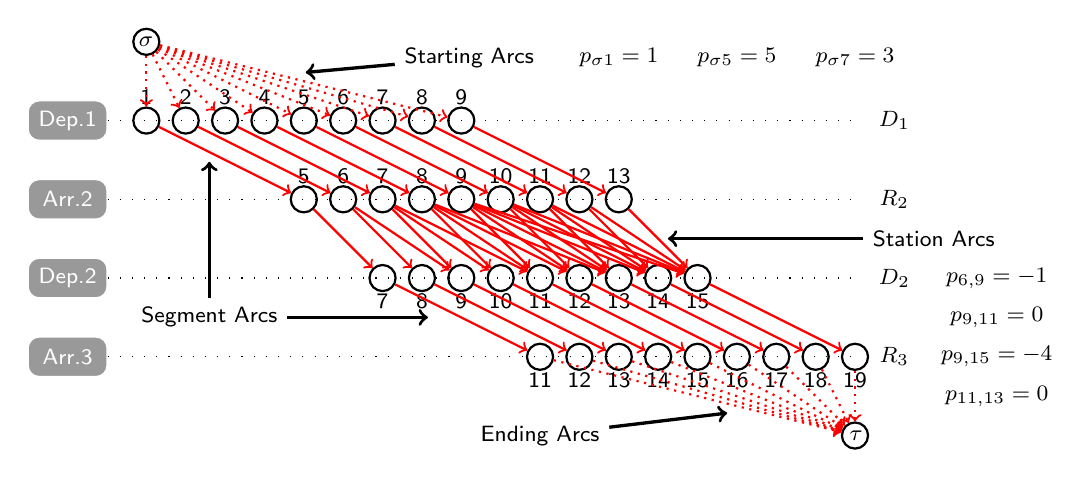
\begin{tikzpicture}
\tikzstyle{every node}=[font=\sffamily\footnotesize]

% minute = 0.5cm

\node (aaa) [xshift=5.5cm,yshift=0.8cm] {$p_{\sigma 1} = 1$};
\node (bbb) [right of=aaa,xshift=0.5cm] {$p_{\sigma 5} = 5$};
\node (ccc) [right of=bbb,xshift=0.5cm] {$p_{\sigma 7} = 3$};
\node (ddd) [xshift=10.3cm,yshift=-2.0cm] {$p_{6,9} = -1$};
\node (eee) [below of=ddd,yshift=0.5cm] {$p_{9,11} = 0$};
\node (fff) [below of=eee,yshift=0.5cm] {$p_{9,15} = -4$};
\node (ggg) [below of=fff,yshift=0.5cm] {$p_{11,13} = 0$};

\node (lbl1) [xshift=3.6cm,yshift=0.8cm] {Starting Arcs};
\node (lbl1e) [left of=lbl1,xshift=-1.2cm,yshift=-0.2cm] {};

\node (lbl2) [xshift=0.3cm,yshift=-2.5cm] {Segment Arcs};
\node (lbl2e) [above of=lbl2,xshift=0cm,yshift=1.1cm] {};
\node (lbl2f) [above of=lbl2,xshift=2.9cm,yshift=-1cm] {};

\node (lbl3) [xshift=9.5cm,yshift=-1.5cm] {Station Arcs};
\node (lbl3e) [left of=lbl3,xshift=-2.5cm] {};

\node (lbl4) [xshift=4.5cm,yshift=-4.0cm] {Ending Arcs};
\node (lbl4e) [right of=lbl4,xshift=1.5cm,yshift=0.3cm] {};

\node (1D)  [nodobianco,xshift=-1.5cm] {Dep.1};
\node (2A)  [nodobianco,below of=1D] {Arr.2};
\node (2D)  [nodobianco,below of=2A,yshift=0.0cm] {Dep.2};
\node (3A)  [nodobianco,below of=2D] {Arr.3};

\node (1De)  [nododummy,right of=1D,xshift=9.5cm] {$D_1$};
\node (2Ae)  [nododummy,right of=2A,xshift=9.5cm] {$R_2$};
\node (2De)  [nododummy,right of=2D,xshift=9.5cm] {$D_2$};
\node (3Ae)  [nododummy,right of=3A,xshift=9.5cm] {$R_3$};

\node (sigma)[eventonero,label={[label distance=-0.4cm]0:{$\sigma$}},above of=1D,xshift=1cm,yshift=0cm] {};
\node (tau)  [eventonero,label={[label distance=-0.4cm]180:{$\tau$}},below of=3A,xshift=10cm,yshift=0cm] {};

\node (D101)[eventonero,label={[label distance=-0.1cm]90:{1}},right of=1D,xshift=0cm,yshift=0cm] {};
\node (D102)[eventonero,label={[label distance=-0.1cm]90:{2}},right of=D101,xshift=-0.5cm,yshift=0cm] {};
\node (D103)[eventonero,label={[label distance=-0.1cm]90:{3}},right of=D102,xshift=-0.5cm,yshift=0cm] {};
\node (D104)[eventonero,label={[label distance=-0.1cm]90:{4}},right of=D103,xshift=-0.5cm,yshift=0cm] {};
\node (D105)[eventonero,label={[label distance=-0.1cm]90:{5}},right of=D104,xshift=-0.5cm,yshift=0cm] {};
\node (D106)[eventonero,label={[label distance=-0.1cm]90:{6}},right of=D105,xshift=-0.5cm,yshift=0cm] {};
\node (D107)[eventonero,label={[label distance=-0.1cm]90:{7}},right of=D106,xshift=-0.5cm,yshift=0cm] {};
\node (D108)[eventonero,label={[label distance=-0.1cm]90:{8}},right of=D107,xshift=-0.5cm,yshift=0cm] {};
\node (D109)[eventonero,label={[label distance=-0.1cm]90:{9}},right of=D108,xshift=-0.5cm,yshift=0cm] {};

\node (A205)[eventonero,label={[label distance=-0.1cm]90:{5}},right of=2A,xshift=2cm,yshift=0cm] {};
\node (A206)[eventonero,label={[label distance=-0.1cm]90:{6}},right of=A205,xshift=-0.5cm,yshift=0cm] {};
\node (A207)[eventonero,label={[label distance=-0.1cm]90:{7}},right of=A206,xshift=-0.5cm,yshift=0cm] {};
\node (A208)[eventonero,label={[label distance=-0.1cm]90:{8}},right of=A207,xshift=-0.5cm,yshift=0cm] {};
\node (A209)[eventonero,label={[label distance=-0.1cm]90:{9}},right of=A208,xshift=-0.5cm,yshift=0cm] {};
\node (A210)[eventonero,label={[label distance=-0.1cm]90:{10}},right of=A209,xshift=-0.5cm,yshift=0cm] {};
\node (A211)[eventonero,label={[label distance=-0.1cm]90:{11}},right of=A210,xshift=-0.5cm,yshift=0cm] {};
\node (A212)[eventonero,label={[label distance=-0.1cm]90:{12}},right of=A211,xshift=-0.5cm,yshift=0cm] {};
\node (A213)[eventonero,label={[label distance=-0.1cm]90:{13}},right of=A212,xshift=-0.5cm,yshift=0cm] {};

\node (D207)[eventonero,label={[label distance=-0.1cm]270:{7}},right of=2D,xshift=3cm,yshift=0cm] {};
\node (D208)[eventonero,label={[label distance=-0.1cm]270:{8}},right of=D207,xshift=-0.5cm,yshift=0cm] {};
\node (D209)[eventonero,label={[label distance=-0.1cm]270:{9}},right of=D208,xshift=-0.5cm,yshift=0cm] {};
\node (D210)[eventonero,label={[label distance=-0.1cm]270:{10}},right of=D209,xshift=-0.5cm,yshift=0cm] {};
\node (D211)[eventonero,label={[label distance=-0.1cm]270:{11}},right of=D210,xshift=-0.5cm,yshift=0cm] {};
\node (D212)[eventonero,label={[label distance=-0.1cm]270:{12}},right of=D211,xshift=-0.5cm,yshift=0cm] {};
\node (D213)[eventonero,label={[label distance=-0.1cm]270:{13}},right of=D212,xshift=-0.5cm,yshift=0cm] {};
\node (D214)[eventonero,label={[label distance=-0.1cm]270:{14}},right of=D213,xshift=-0.5cm,yshift=0cm] {};
\node (D215)[eventonero,label={[label distance=-0.1cm]270:{15}},right of=D214,xshift=-0.5cm,yshift=0cm] {};

\node (A311)[eventonero,label={[label distance=-0.1cm]270:{11}},right of=3A,xshift=5cm,yshift=0cm] {};
\node (A312)[eventonero,label={[label distance=-0.1cm]270:{12}},right of=A311,xshift=-0.5cm,yshift=0cm] {};
\node (A313)[eventonero,label={[label distance=-0.1cm]270:{13}},right of=A312,xshift=-0.5cm,yshift=0cm] {};
\node (A314)[eventonero,label={[label distance=-0.1cm]270:{14}},right of=A313,xshift=-0.5cm,yshift=0cm] {};
\node (A315)[eventonero,label={[label distance=-0.1cm]270:{15}},right of=A314,xshift=-0.5cm,yshift=0cm] {};
\node (A316)[eventonero,label={[label distance=-0.1cm]270:{16}},right of=A315,xshift=-0.5cm,yshift=0cm] {};
\node (A317)[eventonero,label={[label distance=-0.1cm]270:{17}},right of=A316,xshift=-0.5cm,yshift=0cm] {};
\node (A318)[eventonero,label={[label distance=-0.1cm]270:{18}},right of=A317,xshift=-0.5cm,yshift=0cm] {};
\node (A319)[eventonero,label={[label distance=-0.1cm]270:{19}},right of=A318,xshift=-0.5cm,yshift=0cm] {};

%\draw[dotted] or \draw[densely dotted] or \draw[loosely dotted]

\draw[very thick,->] (lbl1) -- (lbl1e);
\draw[very thick,->] (lbl2) -- (lbl2e);
\draw[very thick,->] (lbl2) -- (lbl2f);
\draw[very thick,->] (lbl3) -- (lbl3e);
\draw[very thick,->] (lbl4) -- (lbl4e);

\draw[loosely dotted] (1D) -- (1De);
\draw[loosely dotted] (2A) -- (2Ae);
\draw[loosely dotted] (2D) -- (2De);
\draw[loosely dotted] (3A) -- (3Ae);

\draw[red,thick,dotted,->] (sigma) -- (D101);
\draw[red,thick,dotted,->] (sigma) -- (D102);
\draw[red,thick,dotted,->] (sigma) -- (D103);
\draw[red,thick,dotted,->] (sigma) -- (D104);
\draw[red,thick,dotted,->] (sigma) -- (D105);
\draw[red,thick,dotted,->] (sigma) -- (D106);
\draw[red,thick,dotted,->] (sigma) -- (D107);
\draw[red,thick,dotted,->] (sigma) -- (D108);
\draw[red,thick,dotted,->] (sigma) -- (D109);
\draw[red,thick,->] (D101) -- (A205);
\draw[red,thick,->] (D102) -- (A206);
\draw[red,thick,->] (D103) -- (A207);
\draw[red,thick,->] (D104) -- (A208);
\draw[red,thick,->] (D105) -- (A209);
\draw[red,thick,->] (D106) -- (A210);
\draw[red,thick,->] (D107) -- (A211);
\draw[red,thick,->] (D108) -- (A212);
\draw[red,thick,->] (D109) -- (A213);
\draw[red,thick,->] (A205) -- (D207);
\draw[red,thick,->] (A206) -- (D208);
\draw[red,thick,->] (A206) -- (D209);
\draw[red,thick,->] (A207) -- (D209);
\draw[red,thick,->] (A207) -- (D210);
\draw[red,thick,->] (A207) -- (D211);
\draw[red,thick,->] (A208) -- (D210);
\draw[red,thick,->] (A208) -- (D211);
\draw[red,thick,->] (A208) -- (D212);
\draw[red,thick,->] (A208) -- (D213);
\draw[red,thick,->] (A209) -- (D211);
\draw[red,thick,->] (A209) -- (D212);
\draw[red,thick,->] (A209) -- (D213);
\draw[red,thick,->] (A209) -- (D214);
\draw[red,thick,->] (A209) -- (D215);
\draw[red,thick,->] (A210) -- (D212);
\draw[red,thick,->] (A210) -- (D213);
\draw[red,thick,->] (A210) -- (D214);
\draw[red,thick,->] (A210) -- (D215);
\draw[red,thick,->] (A211) -- (D213);
\draw[red,thick,->] (A211) -- (D214);
\draw[red,thick,->] (A211) -- (D215);
\draw[red,thick,->] (A212) -- (D214);
\draw[red,thick,->] (A212) -- (D215);
\draw[red,thick,->] (A213) -- (D215);
\draw[red,thick,->] (D207) -- (A311);
\draw[red,thick,->] (D208) -- (A312);
\draw[red,thick,->] (D209) -- (A313);
\draw[red,thick,->] (D210) -- (A314);
\draw[red,thick,->] (D211) -- (A315);
\draw[red,thick,->] (D212) -- (A316);
\draw[red,thick,->] (D213) -- (A317);
\draw[red,thick,->] (D214) -- (A318);
\draw[red,thick,->] (D215) -- (A319);
\draw[red,thick,dotted,->] (A311) -- (tau);
\draw[red,thick,dotted,->] (A312) -- (tau);
\draw[red,thick,dotted,->] (A313) -- (tau);
\draw[red,thick,dotted,->] (A314) -- (tau);
\draw[red,thick,dotted,->] (A315) -- (tau);
\draw[red,thick,dotted,->] (A316) -- (tau);
\draw[red,thick,dotted,->] (A317) -- (tau);
\draw[red,thick,dotted,->] (A318) -- (tau);
\draw[red,thick,dotted,->] (A319) -- (tau);

\end{tikzpicture}
\end{center}
}
\end{document}


\frame{
\frametitle{Example of Space-Time Graph: Train C}

\begin{columns}
\begin{column}{0.4\textwidth}
\vspace{-0.8cm}
\begin{table}
\begin{scriptsize}
\setlength{\tabcolsep}{4.5pt}
\renewcommand{\arraystretch}{1.2}
\begin{center}
\begin{tabular}{lrrr}
\multicolumn{4}{c}{\bf \colorbox{black}{\bfseries\textcolor{white}{Ideal Profits and Shift/Stretch Penalties}}} \\
\toprule
 & \bf \textcolor{blue}{Train A} & \bf \textcolor{red}{Train B} & \bf \textcolor{brown}{Train C} \\
\cmidrule(lr){2-2} \cmidrule(lr){3-3} \cmidrule(lr){4-4}
Ideal profit $pr_j$          & 4 & 5 & 3 \\
Shift penalty $\pi_j^{sh}$   & 1 & 1 & 1 \\
Stretch penalty $\pi_j^{st}$ & - & 1 & - \\
\bottomrule
\end{tabular}
\end{center}
\end{scriptsize}
\end{table}
\end{column}
\begin{column}{0.6\textwidth}
\begin{table}
\begin{scriptsize}
\setlength{\tabcolsep}{3pt}
\renewcommand{\arraystretch}{1.2}
\begin{center}
\begin{tabular}{lrrrrrr}
\multicolumn{7}{c}{\bf \colorbox{black}{\bfseries\textcolor{white}{Ideal Timetables}}} \\
\toprule
 & \multicolumn{2}{c}{\bf \textcolor{blue}{Train A}} & \multicolumn{2}{c}{\bf \textcolor{red}{Train B}} & \multicolumn{2}{c}{\bf \textcolor{brown}{Train C}} \\
\cmidrule(lr){2-3} \cmidrule(lr){4-5} \cmidrule(lr){6-7}
\bf Station & \bf Arr & \bf Dep & \bf Arr & \bf Dep & \bf Arr & \bf Dep \\
\cmidrule(lr){1-7}
1       &      & 9:10 &      & 9:05 &      &      \\
2       & 9:15 &      & 9:09 & 9:11 &      & 9:08 \\
3       &      &      & 9:15 &      & 9:13 &      \\
\bottomrule
\end{tabular}
\end{center}
\end{scriptsize}
\end{table}
\end{column}
\end{columns}
\vspace{-0.5cm}
\begin{center}
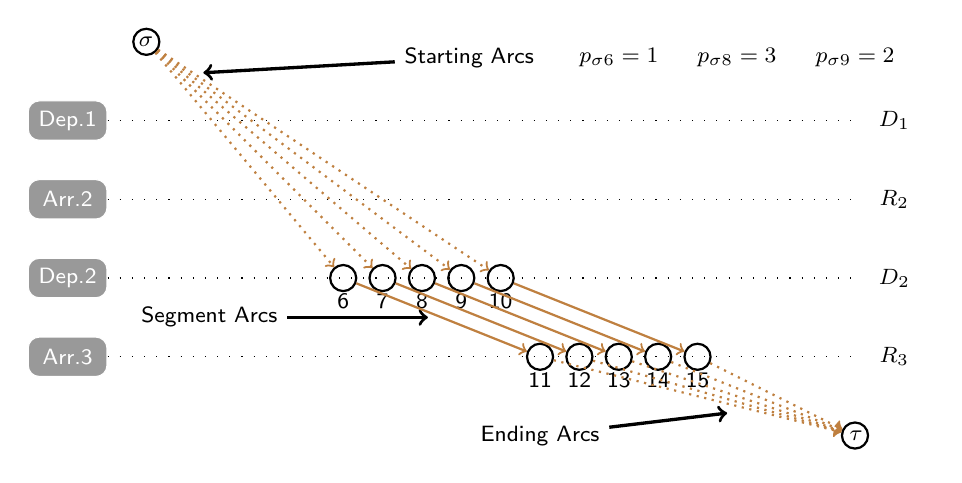
\begin{tikzpicture}
\tikzstyle{every node}=[font=\sffamily\footnotesize]

% minute = 0.5cm

\node (aaa) [xshift=5.5cm,yshift=0.8cm] {$p_{\sigma 6} = 1$};
\node (bbb) [right of=aaa,xshift=0.5cm] {$p_{\sigma 8} = 3$};
\node (ccc) [right of=bbb,xshift=0.5cm] {$p_{\sigma 9} = 2$};

\node (lbl1) [xshift=3.6cm,yshift=0.8cm] {Starting Arcs};
\node (lbl1e) [left of=lbl1,xshift=-2.5cm,yshift=-0.2cm] {};

\node (lbl2) [xshift=0.3cm,yshift=-2.5cm] {Segment Arcs};
\node (lbl2f) [above of=lbl2,xshift=2.9cm,yshift=-1cm] {};

\node (lbl4) [xshift=4.5cm,yshift=-4.0cm] {Ending Arcs};
\node (lbl4e) [right of=lbl4,xshift=1.5cm,yshift=0.3cm] {};

\node (1D)  [nodobianco,xshift=-1.5cm] {Dep.1};
\node (2A)  [nodobianco,below of=1D] {Arr.2};
\node (2D)  [nodobianco,below of=2A,yshift=0.0cm] {Dep.2};
\node (3A)  [nodobianco,below of=2D] {Arr.3};

\node (1De)  [nododummy,right of=1D,xshift=9.5cm] {$D_1$};
\node (2Ae)  [nododummy,right of=2A,xshift=9.5cm] {$R_2$};
\node (2De)  [nododummy,right of=2D,xshift=9.5cm] {$D_2$};
\node (3Ae)  [nododummy,right of=3A,xshift=9.5cm] {$R_3$};

\node (sigma)[eventonero,label={[label distance=-0.4cm]0:{$\sigma$}},above of=1D,xshift=1cm,yshift=0cm] {};
\node (tau)  [eventonero,label={[label distance=-0.4cm]180:{$\tau$}},below of=3A,xshift=10cm,yshift=0cm] {};

\node (D206)[eventonero,label={[label distance=-0.1cm]270:{6}},right of=2D,xshift=2.5cm,yshift=0cm] {};
\node (D207)[eventonero,label={[label distance=-0.1cm]270:{7}},right of=D206,xshift=-0.5cm,yshift=0cm] {};
\node (D208)[eventonero,label={[label distance=-0.1cm]270:{8}},right of=D207,xshift=-0.5cm,yshift=0cm] {};
\node (D209)[eventonero,label={[label distance=-0.1cm]270:{9}},right of=D208,xshift=-0.5cm,yshift=0cm] {};
\node (D210)[eventonero,label={[label distance=-0.1cm]270:{10}},right of=D209,xshift=-0.5cm,yshift=0cm] {};

\node (A311)[eventonero,label={[label distance=-0.1cm]270:{11}},right of=3A,xshift=5cm,yshift=0cm] {};
\node (A312)[eventonero,label={[label distance=-0.1cm]270:{12}},right of=A311,xshift=-0.5cm,yshift=0cm] {};
\node (A313)[eventonero,label={[label distance=-0.1cm]270:{13}},right of=A312,xshift=-0.5cm,yshift=0cm] {};
\node (A314)[eventonero,label={[label distance=-0.1cm]270:{14}},right of=A313,xshift=-0.5cm,yshift=0cm] {};
\node (A315)[eventonero,label={[label distance=-0.1cm]270:{15}},right of=A314,xshift=-0.5cm,yshift=0cm] {};

%\draw[dotted] or \draw[densely dotted] or \draw[loosely dotted]

\draw[very thick,->] (lbl1) -- (lbl1e);
\draw[very thick,->] (lbl2) -- (lbl2f);
\draw[very thick,->] (lbl4) -- (lbl4e);

\draw[loosely dotted] (1D) -- (1De);
\draw[loosely dotted] (2A) -- (2Ae);
\draw[loosely dotted] (2D) -- (2De);
\draw[loosely dotted] (3A) -- (3Ae);

\draw[brown,thick,dotted,->] (sigma) -- (D206);
\draw[brown,thick,dotted,->] (sigma) -- (D207);
\draw[brown,thick,dotted,->] (sigma) -- (D208);
\draw[brown,thick,dotted,->] (sigma) -- (D209);
\draw[brown,thick,dotted,->] (sigma) -- (D210);
\draw[brown,thick,->] (D206) -- (A311);
\draw[brown,thick,->] (D207) -- (A312);
\draw[brown,thick,->] (D208) -- (A313);
\draw[brown,thick,->] (D209) -- (A314);
\draw[brown,thick,->] (D210) -- (A315);
\draw[brown,thick,dotted,->] (A311) -- (tau);
\draw[brown,thick,dotted,->] (A312) -- (tau);
\draw[brown,thick,dotted,->] (A313) -- (tau);
\draw[brown,thick,dotted,->] (A314) -- (tau);
\draw[brown,thick,dotted,->] (A315) -- (tau);
\end{tikzpicture}
\end{center}
}

\frame{
\frametitle{Example of Space-Time Graph}

\begin{columns}
\begin{column}{0.4\textwidth}
\vspace{-0.8cm}
\begin{table}
\begin{scriptsize}
\setlength{\tabcolsep}{4.5pt}
\renewcommand{\arraystretch}{1.2}
\begin{center}
\begin{tabular}{lrrr}
\multicolumn{4}{c}{\bf \colorbox{black}{\bfseries\textcolor{white}{Ideal Profits and Shift/Stretch Penalties}}} \\
\toprule
 & \bf \textcolor{blue}{Train A} & \bf \textcolor{red}{Train B} & \bf \textcolor{brown}{Train C} \\
\cmidrule(lr){2-2} \cmidrule(lr){3-3} \cmidrule(lr){4-4}
Ideal profit $pr_j$          & 4 & 5 & 3 \\
Shift penalty $\pi_j^{sh}$   & 1 & 1 & 1 \\
Stretch penalty $\pi_j^{st}$ & - & 1 & - \\
\bottomrule
\end{tabular}
\end{center}
\end{scriptsize}
\end{table}
\end{column}
\begin{column}{0.6\textwidth}
\begin{table}
\begin{scriptsize}
\setlength{\tabcolsep}{3pt}
\renewcommand{\arraystretch}{1.2}
\begin{center}
\begin{tabular}{lrrrrrr}
\multicolumn{7}{c}{\bf \colorbox{black}{\bfseries\textcolor{white}{Ideal Timetables}}} \\
\toprule
 & \multicolumn{2}{c}{\bf \textcolor{blue}{Train A}} & \multicolumn{2}{c}{\bf \textcolor{red}{Train B}} & \multicolumn{2}{c}{\bf \textcolor{brown}{Train C}} \\
\cmidrule(lr){2-3} \cmidrule(lr){4-5} \cmidrule(lr){6-7}
\bf Station & \bf Arr & \bf Dep & \bf Arr & \bf Dep & \bf Arr & \bf Dep \\
\cmidrule(lr){1-7}
1       &      & 9:10 &      & 9:05 &      &      \\
2       & 9:15 &      & 9:09 & 9:11 &      & 9:08 \\
3       &      &      & 9:15 &      & 9:13 &      \\
\bottomrule
\end{tabular}
\end{center}
\end{scriptsize}
\end{table}
\end{column}
\end{columns}
\vspace{-0.5cm}
\begin{center}
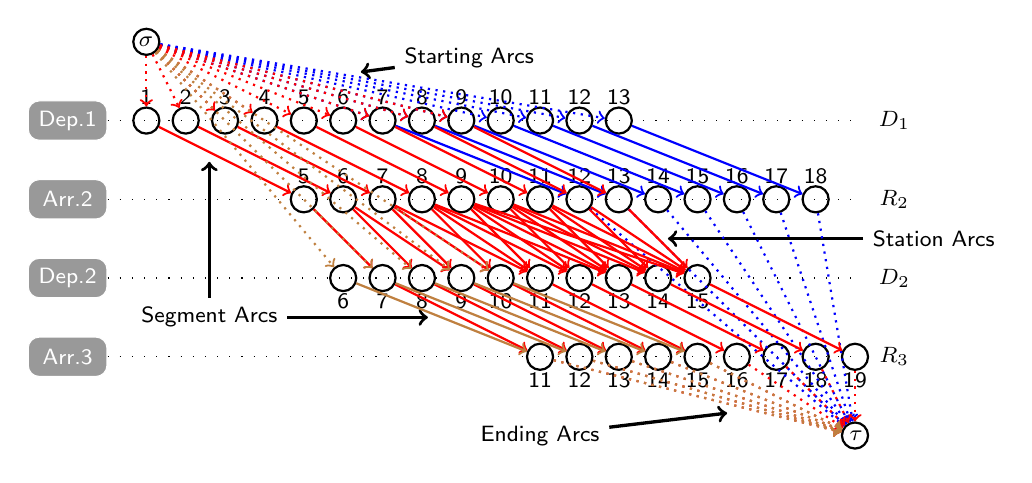
\begin{tikzpicture}
\tikzstyle{every node}=[font=\sffamily\footnotesize]

% minute = 0.5cm

\node (lbl1) [xshift=3.6cm,yshift=0.8cm] {Starting Arcs};
\node (lbl1e) [left of=lbl1,xshift=-0.5cm,yshift=-0.2cm] {};

\node (lbl2) [xshift=0.3cm,yshift=-2.5cm] {Segment Arcs};
\node (lbl2e) [above of=lbl2,xshift=0cm,yshift=1.1cm] {};
\node (lbl2f) [above of=lbl2,xshift=2.9cm,yshift=-1cm] {};

\node (lbl3) [xshift=9.5cm,yshift=-1.5cm] {Station Arcs};
\node (lbl3e) [left of=lbl3,xshift=-2.5cm] {};

\node (lbl4) [xshift=4.5cm,yshift=-4.0cm] {Ending Arcs};
\node (lbl4e) [right of=lbl4,xshift=1.5cm,yshift=0.3cm] {};

\node (1D)  [nodobianco,xshift=-1.5cm] {Dep.1};
\node (2A)  [nodobianco,below of=1D] {Arr.2};
\node (2D)  [nodobianco,below of=2A,yshift=0.0cm] {Dep.2};
\node (3A)  [nodobianco,below of=2D] {Arr.3};

\node (1De)  [nododummy,right of=1D,xshift=9.5cm] {$D_1$};
\node (2Ae)  [nododummy,right of=2A,xshift=9.5cm] {$R_2$};
\node (2De)  [nododummy,right of=2D,xshift=9.5cm] {$D_2$};
\node (3Ae)  [nododummy,right of=3A,xshift=9.5cm] {$R_3$};

\node (sigma)[eventonero,label={[label distance=-0.4cm]0:{$\sigma$}},above of=1D,xshift=1cm,yshift=0cm] {};
\node (tau)  [eventonero,label={[label distance=-0.4cm]180:{$\tau$}},below of=3A,xshift=10cm,yshift=0cm] {};

\node (D101)[eventonero,label={[label distance=-0.1cm]90:{1}},right of=1D,xshift=0cm,yshift=0cm] {};
\node (D102)[eventonero,label={[label distance=-0.1cm]90:{2}},right of=D101,xshift=-0.5cm,yshift=0cm] {};
\node (D103)[eventonero,label={[label distance=-0.1cm]90:{3}},right of=D102,xshift=-0.5cm,yshift=0cm] {};
\node (D104)[eventonero,label={[label distance=-0.1cm]90:{4}},right of=D103,xshift=-0.5cm,yshift=0cm] {};
\node (D105)[eventonero,label={[label distance=-0.1cm]90:{5}},right of=D104,xshift=-0.5cm,yshift=0cm] {};
\node (D106)[eventonero,label={[label distance=-0.1cm]90:{6}},right of=D105,xshift=-0.5cm,yshift=0cm] {};
\node (D107)[eventonero,label={[label distance=-0.1cm]90:{7}},right of=D106,xshift=-0.5cm,yshift=0cm] {};
\node (D108)[eventonero,label={[label distance=-0.1cm]90:{8}},right of=D107,xshift=-0.5cm,yshift=0cm] {};
\node (D109)[eventonero,label={[label distance=-0.1cm]90:{9}},right of=D108,xshift=-0.5cm,yshift=0cm] {};
\node (D110)[eventonero,label={[label distance=-0.1cm]90:{10}},right of=D109,xshift=-0.5cm,yshift=0cm] {};
\node (D111)[eventonero,label={[label distance=-0.1cm]90:{11}},right of=D110,xshift=-0.5cm,yshift=0cm] {};
\node (D112)[eventonero,label={[label distance=-0.1cm]90:{12}},right of=D111,xshift=-0.5cm,yshift=0cm] {};
\node (D113)[eventonero,label={[label distance=-0.1cm]90:{13}},right of=D112,xshift=-0.5cm,yshift=0cm] {};

\node (A205)[eventonero,label={[label distance=-0.1cm]90:{5}},right of=2A,xshift=2cm,yshift=0cm] {};
\node (A206)[eventonero,label={[label distance=-0.1cm]90:{6}},right of=A205,xshift=-0.5cm,yshift=0cm] {};
\node (A207)[eventonero,label={[label distance=-0.1cm]90:{7}},right of=A206,xshift=-0.5cm,yshift=0cm] {};
\node (A208)[eventonero,label={[label distance=-0.1cm]90:{8}},right of=A207,xshift=-0.5cm,yshift=0cm] {};
\node (A209)[eventonero,label={[label distance=-0.1cm]90:{9}},right of=A208,xshift=-0.5cm,yshift=0cm] {};
\node (A210)[eventonero,label={[label distance=-0.1cm]90:{10}},right of=A209,xshift=-0.5cm,yshift=0cm] {};
\node (A211)[eventonero,label={[label distance=-0.1cm]90:{11}},right of=A210,xshift=-0.5cm,yshift=0cm] {};
\node (A212)[eventonero,label={[label distance=-0.1cm]90:{12}},right of=A211,xshift=-0.5cm,yshift=0cm] {};
\node (A213)[eventonero,label={[label distance=-0.1cm]90:{13}},right of=A212,xshift=-0.5cm,yshift=0cm] {};
\node (A214)[eventonero,label={[label distance=-0.1cm]90:{14}},right of=A213,xshift=-0.5cm,yshift=0cm] {};
\node (A215)[eventonero,label={[label distance=-0.1cm]90:{15}},right of=A214,xshift=-0.5cm,yshift=0cm] {};
\node (A216)[eventonero,label={[label distance=-0.1cm]90:{16}},right of=A215,xshift=-0.5cm,yshift=0cm] {};
\node (A217)[eventonero,label={[label distance=-0.1cm]90:{17}},right of=A216,xshift=-0.5cm,yshift=0cm] {};
\node (A218)[eventonero,label={[label distance=-0.1cm]90:{18}},right of=A217,xshift=-0.5cm,yshift=0cm] {};

\node (D206)[eventonero,label={[label distance=-0.1cm]270:{6}},right of=2D,xshift=2.5cm,yshift=0cm] {};
\node (D207)[eventonero,label={[label distance=-0.1cm]270:{7}},right of=D206,xshift=-0.5cm,yshift=0cm] {};
\node (D208)[eventonero,label={[label distance=-0.1cm]270:{8}},right of=D207,xshift=-0.5cm,yshift=0cm] {};
\node (D209)[eventonero,label={[label distance=-0.1cm]270:{9}},right of=D208,xshift=-0.5cm,yshift=0cm] {};
\node (D210)[eventonero,label={[label distance=-0.1cm]270:{10}},right of=D209,xshift=-0.5cm,yshift=0cm] {};
\node (D211)[eventonero,label={[label distance=-0.1cm]270:{11}},right of=D210,xshift=-0.5cm,yshift=0cm] {};
\node (D212)[eventonero,label={[label distance=-0.1cm]270:{12}},right of=D211,xshift=-0.5cm,yshift=0cm] {};
\node (D213)[eventonero,label={[label distance=-0.1cm]270:{13}},right of=D212,xshift=-0.5cm,yshift=0cm] {};
\node (D214)[eventonero,label={[label distance=-0.1cm]270:{14}},right of=D213,xshift=-0.5cm,yshift=0cm] {};
\node (D215)[eventonero,label={[label distance=-0.1cm]270:{15}},right of=D214,xshift=-0.5cm,yshift=0cm] {};

\node (A311)[eventonero,label={[label distance=-0.1cm]270:{11}},right of=3A,xshift=5cm,yshift=0cm] {};
\node (A312)[eventonero,label={[label distance=-0.1cm]270:{12}},right of=A311,xshift=-0.5cm,yshift=0cm] {};
\node (A313)[eventonero,label={[label distance=-0.1cm]270:{13}},right of=A312,xshift=-0.5cm,yshift=0cm] {};
\node (A314)[eventonero,label={[label distance=-0.1cm]270:{14}},right of=A313,xshift=-0.5cm,yshift=0cm] {};
\node (A315)[eventonero,label={[label distance=-0.1cm]270:{15}},right of=A314,xshift=-0.5cm,yshift=0cm] {};
\node (A316)[eventonero,label={[label distance=-0.1cm]270:{16}},right of=A315,xshift=-0.5cm,yshift=0cm] {};
\node (A317)[eventonero,label={[label distance=-0.1cm]270:{17}},right of=A316,xshift=-0.5cm,yshift=0cm] {};
\node (A318)[eventonero,label={[label distance=-0.1cm]270:{18}},right of=A317,xshift=-0.5cm,yshift=0cm] {};
\node (A319)[eventonero,label={[label distance=-0.1cm]270:{19}},right of=A318,xshift=-0.5cm,yshift=0cm] {};

%\draw[dotted] or \draw[densely dotted] or \draw[loosely dotted]

\draw[very thick,->] (lbl1) -- (lbl1e);
\draw[very thick,->] (lbl2) -- (lbl2e);
\draw[very thick,->] (lbl2) -- (lbl2f);
\draw[very thick,->] (lbl3) -- (lbl3e);
\draw[very thick,->] (lbl4) -- (lbl4e);

\draw[loosely dotted] (1D) -- (1De);
\draw[loosely dotted] (2A) -- (2Ae);
\draw[loosely dotted] (2D) -- (2De);
\draw[loosely dotted] (3A) -- (3Ae);

\draw[blue,thick,dotted,->] (sigma) -- (D107);
\draw[blue,thick,dotted,->] (sigma) -- (D108);
\draw[blue,thick,dotted,->] (sigma) -- (D109);
\draw[blue,thick,dotted,->] (sigma) -- (D110);
\draw[blue,thick,dotted,->] (sigma) -- (D111);
\draw[blue,thick,dotted,->] (sigma) -- (D112);
\draw[blue,thick,dotted,->] (sigma) -- (D113);
\draw[blue,thick,->] (D107) -- (A212);
\draw[blue,thick,->] (D108) -- (A213);
\draw[blue,thick,->] (D109) -- (A214);
\draw[blue,thick,->] (D110) -- (A215);
\draw[blue,thick,->] (D111) -- (A216);
\draw[blue,thick,->] (D112) -- (A217);
\draw[blue,thick,->] (D113) -- (A218);
\draw[blue,thick,dotted,->] (A212) -- (tau);
\draw[blue,thick,dotted,->] (A213) -- (tau);
\draw[blue,thick,dotted,->] (A214) -- (tau);
\draw[blue,thick,dotted,->] (A215) -- (tau);
\draw[blue,thick,dotted,->] (A216) -- (tau);
\draw[blue,thick,dotted,->] (A217) -- (tau);
\draw[blue,thick,dotted,->] (A218) -- (tau);

\draw[red,thick,dotted,->] (sigma) -- (D101);
\draw[red,thick,dotted,->] (sigma) -- (D102);
\draw[red,thick,dotted,->] (sigma) -- (D103);
\draw[red,thick,dotted,->] (sigma) -- (D104);
\draw[red,thick,dotted,->] (sigma) -- (D105);
\draw[red,thick,dotted,->] (sigma) -- (D106);
\draw[red,thick,dotted,->] (sigma) -- (D107);
\draw[red,thick,dotted,->] (sigma) -- (D108);
\draw[red,thick,dotted,->] (sigma) -- (D109);
\draw[red,thick,->] (D101) -- (A205);
\draw[red,thick,->] (D102) -- (A206);
\draw[red,thick,->] (D103) -- (A207);
\draw[red,thick,->] (D104) -- (A208);
\draw[red,thick,->] (D105) -- (A209);
\draw[red,thick,->] (D106) -- (A210);
\draw[red,thick,->] (D107) -- (A211);
\draw[red,thick,->] (D108) -- (A212);
\draw[red,thick,->] (D109) -- (A213);
\draw[red,thick,->] (A205) -- (D207);
\draw[red,thick,->] (A206) -- (D208);
\draw[red,thick,->] (A206) -- (D209);
\draw[red,thick,->] (A207) -- (D209);
\draw[red,thick,->] (A207) -- (D210);
\draw[red,thick,->] (A207) -- (D211);
\draw[red,thick,->] (A208) -- (D210);
\draw[red,thick,->] (A208) -- (D211);
\draw[red,thick,->] (A208) -- (D212);
\draw[red,thick,->] (A208) -- (D213);
\draw[red,thick,->] (A209) -- (D211);
\draw[red,thick,->] (A209) -- (D212);
\draw[red,thick,->] (A209) -- (D213);
\draw[red,thick,->] (A209) -- (D214);
\draw[red,thick,->] (A209) -- (D215);
\draw[red,thick,->] (A210) -- (D212);
\draw[red,thick,->] (A210) -- (D213);
\draw[red,thick,->] (A210) -- (D214);
\draw[red,thick,->] (A210) -- (D215);
\draw[red,thick,->] (A211) -- (D213);
\draw[red,thick,->] (A211) -- (D214);
\draw[red,thick,->] (A211) -- (D215);
\draw[red,thick,->] (A212) -- (D214);
\draw[red,thick,->] (A212) -- (D215);
\draw[red,thick,->] (A213) -- (D215);
\draw[red,thick,->] (D207) -- (A311);
\draw[red,thick,->] (D208) -- (A312);
\draw[red,thick,->] (D209) -- (A313);
\draw[red,thick,->] (D210) -- (A314);
\draw[red,thick,->] (D211) -- (A315);
\draw[red,thick,->] (D212) -- (A316);
\draw[red,thick,->] (D213) -- (A317);
\draw[red,thick,->] (D214) -- (A318);
\draw[red,thick,->] (D215) -- (A319);
\draw[red,thick,dotted,->] (A311) -- (tau);
\draw[red,thick,dotted,->] (A312) -- (tau);
\draw[red,thick,dotted,->] (A313) -- (tau);
\draw[red,thick,dotted,->] (A314) -- (tau);
\draw[red,thick,dotted,->] (A315) -- (tau);
\draw[red,thick,dotted,->] (A316) -- (tau);
\draw[red,thick,dotted,->] (A317) -- (tau);
\draw[red,thick,dotted,->] (A318) -- (tau);
\draw[red,thick,dotted,->] (A319) -- (tau);

\draw[brown,thick,dotted,->] (sigma) -- (D206);
\draw[brown,thick,dotted,->] (sigma) -- (D207);
\draw[brown,thick,dotted,->] (sigma) -- (D208);
\draw[brown,thick,dotted,->] (sigma) -- (D209);
\draw[brown,thick,dotted,->] (sigma) -- (D210);
\draw[brown,thick,->] (D206) -- (A311);
\draw[brown,thick,->] (D207) -- (A312);
\draw[brown,thick,->] (D208) -- (A313);
\draw[brown,thick,->] (D209) -- (A314);
\draw[brown,thick,->] (D210) -- (A315);
\draw[brown,thick,dotted,->] (A311) -- (tau);
\draw[brown,thick,dotted,->] (A312) -- (tau);
\draw[brown,thick,dotted,->] (A313) -- (tau);
\draw[brown,thick,dotted,->] (A314) -- (tau);
\draw[brown,thick,dotted,->] (A315) -- (tau);
\end{tikzpicture}
\end{center}
}

\frame{
\frametitle{Ideal Timetables and Paths in the Space-Time Graph}

\begin{columns}
\begin{column}{0.4\textwidth}
\vspace{-0.5cm}
\begin{table}
\begin{scriptsize}
\setlength{\tabcolsep}{3.5pt}
\renewcommand{\arraystretch}{1.2}
\begin{center}
\begin{tabular}{lrrr}
\multicolumn{4}{c}{\bf \colorbox{black}{\bfseries\textcolor{white}{Ideal Profits and Shift/Stretch Penalties}}} \\
\toprule
 & \bf \textcolor{blue}{Train A} & \bf \textcolor{red}{Train B} & \bf \textcolor{brown}{Train C} \\
\cmidrule(lr){2-2} \cmidrule(lr){3-3} \cmidrule(lr){4-4}
Ideal profit $pr_j$          & 500 & 500 & 100 \\
Shift penalty $\pi_j^{sh}$   &   1 &   8 &  10 \\
Stretch penalty $\pi_j^{st}$ &   2 &  10 &  20 \\
\bottomrule
\end{tabular}
\end{center}
\end{scriptsize}
\end{table}
\vspace{-0.6cm}
\begin{table}
\begin{scriptsize}
\setlength{\tabcolsep}{4.5pt}
\renewcommand{\arraystretch}{1.2}
\begin{center}
\begin{tabular}{l}
\multicolumn{1}{c}{\bf \colorbox{black}{\bfseries\textcolor{white}{Headway Times}}} \\
\toprule
Departures $h_i^d = 2, \forall i \in S \setminus \{s\}$ \\
Arrivals $h_i^a = 4, \forall i \in S \setminus \{1\}$ \\
\bottomrule
\end{tabular}
\end{center}
\end{scriptsize}
\end{table}
\end{column}
\begin{column}{0.6\textwidth}
\vspace{-0.5cm}
\begin{table}
\begin{scriptsize}
\setlength{\tabcolsep}{3.5pt}
\renewcommand{\arraystretch}{1.2}
\begin{center}
\begin{tabular}{lrrrrrr}
\multicolumn{7}{c}{\bf \colorbox{black}{\bfseries\textcolor{white}{Ideal Timetables}}} \\
\toprule
 & \multicolumn{2}{c}{\bf \textcolor{blue}{Train A}} & \multicolumn{2}{c}{\bf \textcolor{red}{Train B}} & \multicolumn{2}{c}{\bf \textcolor{brown}{Train C}} \\
\cmidrule(lr){2-3} \cmidrule(lr){4-5} \cmidrule(lr){6-7}
\bf Station & \bf Arr & \bf Dep & \bf Arr & \bf Dep & \bf Arr & \bf Dep \\
\cmidrule(lr){1-7}
1       &      & 9:00 &       &  9:00 &       &       \\
2       & 9:05 & 9:07 &  9:10 &  9:12 &       &       \\
3       & 9:18 &      &  9:30 &  9:35 &       &  9:33 \\
4       &      &      & 10:00 & 10:03 & 10:02 & 10:07 \\
5       &      &      & 10:20 &       & 10:24 &       \\
\bottomrule
\end{tabular}
\end{center}
\end{scriptsize}
\end{table}
\end{column}
\end{columns}
\vspace{-0.4cm}
\begin{center}
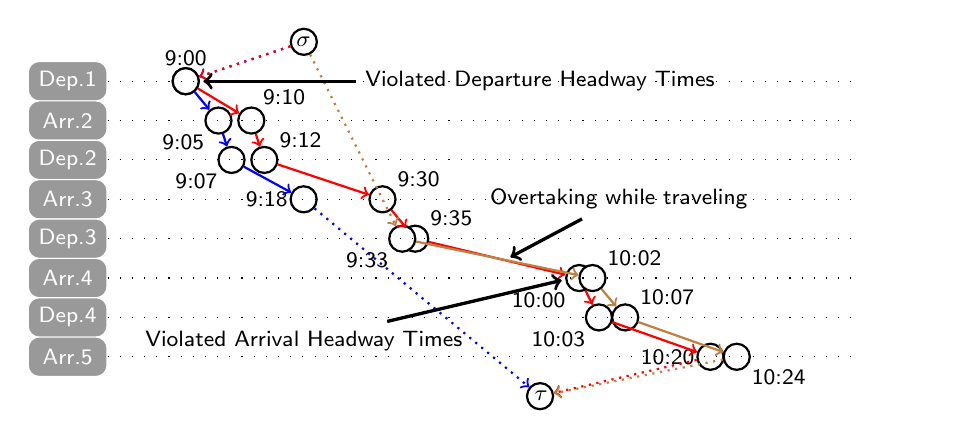
\begin{tikzpicture}
\tikzstyle{every node}=[font=\sffamily\footnotesize]

\node (1D)  [nodobianco,xshift=-1.5cm] {Dep.1};
\node (2A)  [nodobianco,below of=1D,yshift=0.5cm] {Arr.2};
\node (2D)  [nodobianco,below of=2A,yshift=0.5cm] {Dep.2};
\node (3A)  [nodobianco,below of=2D,yshift=0.5cm] {Arr.3};
\node (3D)  [nodobianco,below of=3A,yshift=0.5cm] {Dep.3};
\node (4A)  [nodobianco,below of=3D,yshift=0.5cm] {Arr.4};
\node (4D)  [nodobianco,below of=4A,yshift=0.5cm] {Dep.4};
\node (5A)  [nodobianco,below of=4D,yshift=0.5cm] {Arr.5};

\node (1De)  [nododummy,right of=1D,xshift=9.5cm] {};
\node (2Ae)  [nododummy,right of=2A,xshift=9.5cm] {};
\node (2De)  [nododummy,right of=2D,xshift=9.5cm] {};
\node (3Ae)  [nododummy,right of=3A,xshift=9.5cm] {};
\node (3De)  [nododummy,right of=3D,xshift=9.5cm] {};
\node (4Ae)  [nododummy,right of=4A,xshift=9.5cm] {};
\node (4De)  [nododummy,right of=4D,xshift=9.5cm] {};
\node (5Ae)  [nododummy,right of=5A,xshift=9.5cm] {};

\node (sigma)[eventonero,label={[label distance=-0.4cm]0:{$\sigma$}},above of=1D,xshift=3cm,yshift=-0.5cm] {};
\node (tau)  [eventonero,label={[label distance=-0.4cm]180:{$\tau$}},below of=5A,xshift=6cm,yshift=0.5cm] {};

\node (A_D1) [eventonero,label={[label distance=-0.1cm]90:9:00},right of=1D,xshift=0.5cm] {}; % to fill
\node (A_A2) [eventonero,label={[label distance=-0.1cm]225:9:05},below of=A_D1,xshift=0.416cm,yshift=0.5cm] {};
\node (A_D2) [eventonero,label={[label distance=-0.1cm]225:9:07},below of=A_A2,xshift=0.166cm,yshift=0.5cm] {};
\node (A_A3) [eventonero,label={[label distance=-0.1cm]180:9:18},below of=A_D2,xshift=0.916cm,yshift=0.5cm] {};

\node (B_D1) [eventonero,label={[label distance=-0.1cm]90:},right of=1D,xshift=0.5cm] {};
\node (B_A2) [eventonero,label={[label distance=-0.1cm]70:9:10},below of=B_D1,xshift=0.833cm,yshift=0.5cm] {};
\node (B_D2) [eventonero,label={[label distance=-0.1cm]30:9:12},below of=B_A2,xshift=0.166cm,yshift=0.5cm] {};
\node (B_A3) [eventonero,label={[label distance=-0.1cm]30:9:30},below of=B_D2,xshift=1.5cm,yshift=0.5cm] {};
\node (B_D3) [eventonero,label={[label distance=-0.1cm]30:9:35},below of=B_A3,xshift=0.416cm,yshift=0.5cm] {};
\node (B_A4) [eventonero,label={[label distance=-0.1cm]230:10:00},below of=B_D3,xshift=2.083cm,yshift=0.5cm] {};
\node (B_D4) [eventonero,label={[label distance=-0.1cm]230:10:03},below of=B_A4,xshift=0.25cm,yshift=0.5cm] {};
\node (B_A5) [eventonero,label={[label distance=-0.1cm]180:10:20},below of=B_D4,xshift=1.416cm,yshift=0.5cm] {};

\node (C_D3) [eventonero,label={[label distance=-0.1cm]225:9:33},right of=3D,xshift=3.25cm] {};
\node (C_A4) [eventonero,label={[label distance=-0.1cm]30:10:02},below of=C_D3,xshift=2.416cm,yshift=0.5cm] {};
\node (C_D4) [eventonero,label={[label distance=-0.1cm]30:10:07},below of=C_A4,xshift=0.416cm,yshift=0.5cm] {};
\node (C_A5) [eventonero,label={[label distance=-0.1cm]330:10:24},below of=C_D4,xshift=1.416cm,yshift=0.5cm] {};

%\draw[dotted] or \draw[densely dotted] or \draw[loosely dotted]

\draw[loosely dotted] (1D) -- (1De);
\draw[loosely dotted] (2A) -- (2Ae);
\draw[loosely dotted] (2D) -- (2De);
\draw[loosely dotted] (3A) -- (3Ae);
\draw[loosely dotted] (3D) -- (3De);
\draw[loosely dotted] (4A) -- (4Ae);
\draw[loosely dotted] (4D) -- (4De);
\draw[loosely dotted] (5A) -- (5Ae);

\draw[blue,thick,dotted,->] (sigma) -- (A_D1);
\draw[blue,thick,->] (A_D1) -- (A_A2);
\draw[blue,thick,->] (A_A2) -- (A_D2);
\draw[blue,thick,->] (A_D2) -- (A_A3);
\draw[blue,thick,dotted,->] (A_A3) -- (tau);

\draw[red,thick,dotted,->] (sigma) -- (B_D1);
\draw[red,thick,->] (B_D1) -- (B_A2);
\draw[red,thick,->] (B_A2) -- (B_D2);
\draw[red,thick,->] (B_D2) -- (B_A3);
\draw[red,thick,->] (B_A3) -- (B_D3);
\draw[red,thick,->] (B_D3) -- (B_A4);
\draw[red,thick,->] (B_A4) -- (B_D4);
\draw[red,thick,->] (B_D4) -- (B_A5);
\draw[red,thick,dotted,->] (B_A5) -- (tau);

\draw[brown,thick,dotted,->] (sigma) -- (C_D3);
\draw[brown,thick,->] (C_D3) -- (C_A4);
\draw[brown,thick,->] (C_A4) -- (C_D4);
\draw[brown,thick,->] (C_D4) -- (C_A5);
\draw[brown,thick,dotted,->] (C_A5) -- (tau);

\pause

\node (lbl1) [xshift=5.5cm,yshift=-1.5cm] {Overtaking while traveling};
\node (lbl1e) [left of=lbl1,xshift=-0.5cm,yshift=-0.8cm] {};
\draw[very thick,->] (lbl1) -- (lbl1e);

\pause

\node (lbl2) [xshift=4.5cm,yshift=0cm] {Violated Departure Headway Times};
\node (lbl2e) [left of=lbl2,xshift=-3.4cm] {};
\draw[very thick,->] (lbl2) -- (lbl2e);

\pause

\node (lbl3) [xshift=1.5cm,yshift=-3.3cm] {Violated Arrival Headway Times};
\node (lbl3e) [above of=lbl3,xshift=3.4cm,yshift=-0.2cm] {};
\draw[very thick,->] (lbl3) -- (lbl3e);

\end{tikzpicture}
\end{center}
}

\frame{
\frametitle{Actual Feasible Timetables in the Space-Time Graph}

\begin{columns}
\begin{column}{0.4\textwidth}
\vspace{-0.5cm}
\begin{table}
\begin{scriptsize}
\setlength{\tabcolsep}{3.5pt}
\renewcommand{\arraystretch}{1.2}
\begin{center}
\begin{tabular}{lrrr}
\multicolumn{4}{c}{\bf \colorbox{black}{\bfseries\textcolor{white}{Ideal Profits and Shift/Stretch Penalties}}} \\
\toprule
 & \bf \textcolor{blue}{Train A} & \bf \textcolor{red}{Train B} & \bf \textcolor{brown}{Train C} \\
\cmidrule(lr){2-2} \cmidrule(lr){3-3} \cmidrule(lr){4-4}
Ideal profit $pr_j$          & 500 & 500 & 100 \\
Shift penalty $\pi_j^{sh}$   &   1 &   8 &  10 \\
Stretch penalty $\pi_j^{st}$ &   2 &  10 &  20 \\
\bottomrule
\end{tabular}
\end{center}
\end{scriptsize}
\end{table}
\vspace{-0.6cm}
\begin{table}
\begin{scriptsize}
\setlength{\tabcolsep}{4.5pt}
\renewcommand{\arraystretch}{1.2}
\begin{center}
\begin{tabular}{l}
\multicolumn{1}{c}{\bf \colorbox{black}{\bfseries\textcolor{white}{Headway Times}}} \\
\toprule
Departures $h_i^d = 2, \forall i \in S \setminus \{s\}$ \\
Arrivals $h_i^a = 4, \forall i \in S \setminus \{1\}$ \\
\bottomrule
\end{tabular}
\end{center}
\end{scriptsize}
\end{table}
\end{column}
\begin{column}{0.6\textwidth}
\vspace{-0.5cm}
\begin{table}
\begin{scriptsize}
\setlength{\tabcolsep}{3.5pt}
\renewcommand{\arraystretch}{1.2}
\begin{center}
\begin{tabular}{lrrrrrr}
\multicolumn{7}{c}{\bf \colorbox{black}{\bfseries\textcolor{white}{Actual Timetables}}} \\
\toprule
 & \multicolumn{2}{c}{\bf \textcolor{blue}{Train A}} & \multicolumn{2}{c}{\bf \textcolor{red}{Train B}} & \multicolumn{2}{c}{\bf \textcolor{brown}{Train C}} \\
\cmidrule(lr){2-3} \cmidrule(lr){4-5} \cmidrule(lr){6-7}
\bf Station & \bf Arr & \bf Dep & \bf Arr & \bf Dep & \bf Arr & \bf Dep \\
\cmidrule(lr){1-7}
1       &      & \bf (-2) 8:58 &       &           9:00 &       &       \\
2       & 9:03 &          9:05 &  9:10 &           9:12 &       &       \\
3       & 9:16 &               &  9:30 & \bf (+6)  9:41 &       &  9:33 \\
4       &      &               & 10:06 & \bf (+2) 10:11 & 10:02 & 10:07 \\
5       &      &               & 10:28 &                & 10:24 &       \\
\bottomrule
\end{tabular}
\end{center}
\end{scriptsize}
\end{table}
\end{column}
\end{columns}
\vspace{-0.4cm}
\begin{center}
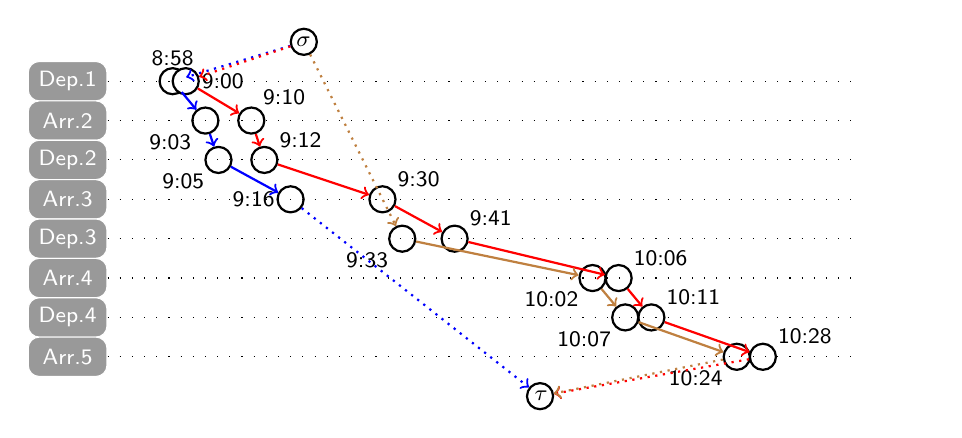
\begin{tikzpicture}
\tikzstyle{every node}=[font=\sffamily\footnotesize]

\node (1D)  [nodobianco,xshift=-1.5cm] {Dep.1};
\node (2A)  [nodobianco,below of=1D,yshift=0.5cm] {Arr.2};
\node (2D)  [nodobianco,below of=2A,yshift=0.5cm] {Dep.2};
\node (3A)  [nodobianco,below of=2D,yshift=0.5cm] {Arr.3};
\node (3D)  [nodobianco,below of=3A,yshift=0.5cm] {Dep.3};
\node (4A)  [nodobianco,below of=3D,yshift=0.5cm] {Arr.4};
\node (4D)  [nodobianco,below of=4A,yshift=0.5cm] {Dep.4};
\node (5A)  [nodobianco,below of=4D,yshift=0.5cm] {Arr.5};

\node (1De)  [nododummy,right of=1D,xshift=9.5cm] {};
\node (2Ae)  [nododummy,right of=2A,xshift=9.5cm] {};
\node (2De)  [nododummy,right of=2D,xshift=9.5cm] {};
\node (3Ae)  [nododummy,right of=3A,xshift=9.5cm] {};
\node (3De)  [nododummy,right of=3D,xshift=9.5cm] {};
\node (4Ae)  [nododummy,right of=4A,xshift=9.5cm] {};
\node (4De)  [nododummy,right of=4D,xshift=9.5cm] {};
\node (5Ae)  [nododummy,right of=5A,xshift=9.5cm] {};

\node (sigma)[eventonero,label={[label distance=-0.4cm]0:{$\sigma$}},above of=1D,xshift=3cm,yshift=-0.5cm] {};
\node (tau)  [eventonero,label={[label distance=-0.4cm]180:{$\tau$}},below of=5A,xshift=6cm,yshift=0.5cm] {};

\node (A_D1) [eventonero,label={[label distance=-0.1cm]90:8:58},right of=1D,xshift=0.334cm] {}; % to fill
\node (A_A2) [eventonero,label={[label distance=-0.1cm]225:9:03},below of=A_D1,xshift=0.416cm,yshift=0.5cm] {};
\node (A_D2) [eventonero,label={[label distance=-0.1cm]225:9:05},below of=A_A2,xshift=0.166cm,yshift=0.5cm] {};
\node (A_A3) [eventonero,label={[label distance=-0.1cm]180:9:16},below of=A_D2,xshift=0.916cm,yshift=0.5cm] {};

\node (B_D1) [eventonero,label={[label distance=-0.1cm]0:9:00},right of=1D,xshift=0.5cm] {};
\node (B_A2) [eventonero,label={[label distance=-0.1cm]70:9:10},below of=B_D1,xshift=0.833cm,yshift=0.5cm] {};
\node (B_D2) [eventonero,label={[label distance=-0.1cm]30:9:12},below of=B_A2,xshift=0.166cm,yshift=0.5cm] {};
\node (B_A3) [eventonero,label={[label distance=-0.1cm]30:9:30},below of=B_D2,xshift=1.5cm,yshift=0.5cm] {};
\node (B_D3) [eventonero,label={[label distance=-0.1cm]30:9:41},below of=B_A3,xshift=0.916cm,yshift=0.5cm] {};
\node (B_A4) [eventonero,label={[label distance=-0.1cm]30:10:06},below of=B_D3,xshift=2.083cm,yshift=0.5cm] {};
\node (B_D4) [eventonero,label={[label distance=-0.1cm]30:10:11},below of=B_A4,xshift=0.416cm,yshift=0.5cm] {};
\node (B_A5) [eventonero,label={[label distance=-0.1cm]30:10:28},below of=B_D4,xshift=1.416cm,yshift=0.5cm] {};

\node (C_D3) [eventonero,label={[label distance=-0.1cm]225:9:33},right of=3D,xshift=3.25cm] {};
\node (C_A4) [eventonero,label={[label distance=-0.1cm]225:10:02},below of=C_D3,xshift=2.416cm,yshift=0.5cm] {};
\node (C_D4) [eventonero,label={[label distance=-0.1cm]225:10:07},below of=C_A4,xshift=0.416cm,yshift=0.5cm] {};
\node (C_A5) [eventonero,label={[label distance=-0.1cm]225:10:24},below of=C_D4,xshift=1.416cm,yshift=0.5cm] {};

%\draw[dotted] or \draw[densely dotted] or \draw[loosely dotted]

\draw[loosely dotted] (1D) -- (1De);
\draw[loosely dotted] (2A) -- (2Ae);
\draw[loosely dotted] (2D) -- (2De);
\draw[loosely dotted] (3A) -- (3Ae);
\draw[loosely dotted] (3D) -- (3De);
\draw[loosely dotted] (4A) -- (4Ae);
\draw[loosely dotted] (4D) -- (4De);
\draw[loosely dotted] (5A) -- (5Ae);

\draw[blue,thick,dotted,->] (sigma) -- (A_D1);
\draw[blue,thick,->] (A_D1) -- (A_A2);
\draw[blue,thick,->] (A_A2) -- (A_D2);
\draw[blue,thick,->] (A_D2) -- (A_A3);
\draw[blue,thick,dotted,->] (A_A3) -- (tau);

\draw[red,thick,dotted,->] (sigma) -- (B_D1);
\draw[red,thick,->] (B_D1) -- (B_A2);
\draw[red,thick,->] (B_A2) -- (B_D2);
\draw[red,thick,->] (B_D2) -- (B_A3);
\draw[red,thick,->] (B_A3) -- (B_D3);
\draw[red,thick,->] (B_D3) -- (B_A4);
\draw[red,thick,->] (B_A4) -- (B_D4);
\draw[red,thick,->] (B_D4) -- (B_A5);
\draw[red,thick,dotted,->] (B_A5) -- (tau);

\draw[brown,thick,dotted,->] (sigma) -- (C_D3);
\draw[brown,thick,->] (C_D3) -- (C_A4);
\draw[brown,thick,->] (C_A4) -- (C_D4);
\draw[brown,thick,->] (C_D4) -- (C_A5);
\draw[brown,thick,dotted,->] (C_A5) -- (tau);

\end{tikzpicture}
\end{center}
}

\section{Mathematical Formulation}

\frame{
\frametitle{Mathematical Model (Cacchiani et al. 2015)}
\begin{block}{Additional Notation}
\begin{tabular}{ll}
\tabitem $\mathcal{P}_j$                           & set of paths of train $j \in T$ \\
\tabitem $P \in \mathcal{P}_j$                     & path from $\sigma$ to $\tau$ made up of arcs of $A_j$, $j \in T$, with a positive profit \\
\tabitem $\mathcal{P}_j^v \subseteq \mathcal{P}_j$ & set of paths of train $j \in T$ that use node $v \in V_j$ \\
\tabitem $\mathcal{P}^v = \cup_{j \in T} \mathcal{P}_j^v$ & set of paths that use node $v \in V$ \\
\tabitem $r_j^i$                                   & travel time of train $j \in T$ from station $i \in S_j \setminus \{l_j\}$ to $i+1 \in S_j$ \\
\end{tabular}
\end{block}
\bigskip
\begin{block}{Variables}
\begin{tabular}{ll}
\tabitem $x_P \in \{0,1\}$ & binary variable equal to 1 if path $P \in \mathcal{P}_j$ of train $j \in T$ is selected \\ 
                           & (0 otherwise) \\
\end{tabular}
\end{block}
}

\frame{
\frametitle{Mathematical Model (Cacchiani et al. 2015)}
\begin{small}
\input{formulation.tex}
\end{small}
}

\frame{
\frametitle{Mathematical Model (Cacchiani et al. 2015)}
\begin{small}
Objective function \eqref{F.0}
$$\max \quad \sum_{j \in T} \sum_{P \in \mathcal{P}_j} \Big( \sum_{a \in P} p_a \Big) x_P$$
$\Rightarrow$ Maximize the profits of the selected paths

\bigskip\bigskip\bigskip

Constraints \eqref{F.1}
$$\sum_{P \in \mathcal{P}_j} x_P \leq 1 \qquad \forall j \in T$$
$\Rightarrow$ Select at most one path for each train $j \in T$
\end{small}
}

\frame{
\frametitle{Mathematical Model (Cacchiani et al. 2015)}
\begin{small}
Constraints \eqref{F.2}
$$\sum_{\substack{w \in R_i \tc\\ 0 \leq \theta(v) - \theta(w) \leq h^a_i-1 }} \sum_{P \in \mathcal{P}^w} x_P \leq 1 \qquad \forall i \in S \setminus \{1\} \quad \forall v \in R_i$$

$\Rightarrow$ \alert{Arrival Time Constraints}: for each node $v \in R_i$ of the space-time graph corresponding to an arrival at station $i \in S \setminus \{1\}$, at most one of the paths arriving at $i$ in the time window $[\theta(v)-h^a_i+1,\theta(v)]$ can be selected

\bigskip\bigskip\bigskip

Constraints \eqref{F.3}
$$\sum_{\substack{w \in D_i \tc\\ 0 \leq \theta(v) - \theta(w) \leq h^d_i-1 }} \sum_{P \in \mathcal{P}^w} x_P \leq 1 \qquad \forall i \in S \setminus \{s\} \quad \forall v \in D_i$$

$\Rightarrow$ \alert{Departure Time Constraints}: for each node $v \in D_i$ of the space-time graph corresponding to a departure from station $i \in S \setminus \{s\}$, at most one of the paths departing from $i$ in the time window $[\theta(v)-h^d_i+1,\theta(v)]$ can be selected
\end{small}
}

\frame{
\frametitle{Mathematical Model: Overtaking Constraints}
\begin{small}
Overtaking constraints \eqref{F.4}: no overtaking can take place while traveling
\begin{alignat*}{3}
           & \sum_{P \in \mathcal{P}_j^v} x_P + \sum_{\substack{w \in D_i \tc\\0 \leq \theta(w) - \theta(v) \leq r_j^i - r_k^i}} \sum_{P \in \mathcal{P}_k^w} x_P \leq 1 & \\
           & \qquad \forall i \in S \setminus \{s\} \quad \forall v \in D_i \quad \forall j,k \in T & \tc j \neq k, \; i,i+1 \in S_j \cap S_k, \; r_j^i \geq r_k^i \\
\end{alignat*}
\vspace{-1.0cm}
\begin{itemize}
\item Consider a time instant corresponding to $v \in D_i$ of departing station $i \in S \setminus \{s\}$
\item Consider two different trains $j, k \in T$ ($j \neq k$) such that both visit stations $i$ and $i+1$ (i.e., $i,i+1 \in S_j \cap S_k$) and such that train $j$ is slower than train $k$ ($r_j^i \geq r_k^i$) when traveling from $i$ to $i+1$
\end{itemize}
\vspace{-0.4cm}
\begin{columns}
\begin{column}{0.6\textwidth}
\begin{itemize}
\item At most one of the next paths can be selected:
\begin{itemize}
\item Paths of train $j$ using node $v$
\item Paths of train $k$ departing from $i$ at time instant $\theta(w)$ with $\theta(w) \geq \theta(v)$ and $\theta(w) + r_k^i \leq \theta(v) + r_j^i$
\end{itemize}
\end{itemize}
\end{column}
\begin{column}{0.4\textwidth}
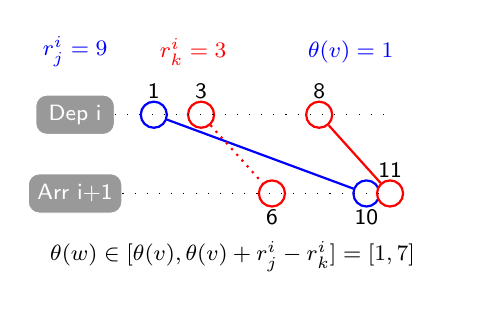
\begin{tikzpicture}
\tikzstyle{every node}=[font=\sffamily\footnotesize]

\node (1D)  [nodobianco] {Dep i};
\node (2A)  [nodobianco,below of=1D] {Arr i+1};

\node (1De)  [nododummy,right of=1D,xshift=3.5cm] {};
\node (2Ae)  [nododummy,right of=2A,xshift=3.5cm] {};

\node (A_D1) [eventoblue,label={[label distance=-0.1cm]90:1},right of=1D,xshift=0.0cm] {}; % to fill
\node (A_A2) [eventoblue,label={[label distance=-0.1cm]270:10},below of=A_D1,xshift=2.7cm] {};

\node (B_D1) [eventorosso,label={[label distance=-0.1cm]90:3},right of=1D,xshift=0.6cm] {};
\node (B_A2) [eventorosso,label={[label distance=-0.1cm]270:6},below of=B_D1,xshift=0.9cm] {};

\node (B_D12) [eventorosso,label={[label distance=-0.1cm]90:8},right of=1D,xshift=2.1cm] {};
\node (B_A22) [eventorosso,label={[label distance=-0.1cm]90:11},below of=B_D12,xshift=0.9cm] {};

\draw[loosely dotted] (1D) -- (1De);
\draw[loosely dotted] (2A) -- (2Ae);

\draw[blue,thick] (A_D1) -- (A_A2);

\draw[red,thick,dotted] (B_D1) -- (B_A2);
\draw[red,thick] (B_D12) -- (B_A22);

\node (j) [xshift=0.0cm,yshift=0.8cm] {\textcolor{blue}{$r_j^i = 9$}};
\node (k) [xshift=1.5cm,yshift=0.8cm] {\textcolor{red}{$r_k^i = 3$}};
\node (j) [xshift=3.5cm,yshift=0.8cm] {\textcolor{blue}{$\theta(v) = 1$}};

\node (j) [xshift=2.0cm,yshift=-1.8cm] {$\theta(w) \in [\theta(v),\theta(v)+r_j^i-r_k^i] = [1,7]$};
\end{tikzpicture}
\end{column}
\end{columns}
\end{small}
}

\frame{
\frametitle{Mathematical Model: Comments}
\begin{itemize}
\item Different paths-based models can be written: the main differences lie in the way constraints are expressed
\item The presented formulation has the disadvantage of having exponentially many variables that rapidly grow with the number of stations and the length of the planning horizon
\item Even the number of constraints rapidly grows with the number of stations and the length of the planning horizon
\item Solution methods based on paths-based models rely on column generation
\item Effective branch-and-cut-and-price algorithms can be developed for small/medium-size instances
\item For large instances, good heuristic solutions can be found with LP-based heuristic procedures
\end{itemize}
}

\section{Conclusions}

\frame{
\frametitle{Final Comments}
\begin{itemize}
\item We have considered TTPs, which is the second phase of optimization of passenger railway systems
\item The goal is to define the timetables (arrival and departure times at each visited station) of each train while maximizing the profit of Train Operators
\item We have considered a limited number of constraints arising in practical applications
\item A common way of representing TTPs is through space-time graphs
\item We have formulated TTPs with a path-based mathematical formulation
\item In practice, only small-medium size instances can be solved to optimality with path-based formulations; for large instances, only heuristic solutions can be found
\end{itemize}
}

\section{}

\newcommand\contactTable{
  \begin{tabular}{lr}
    \multicolumn{2}{l}{Roberto Roberti} \\ 
    \multicolumn{2}{l}{Department of Transport, Technical University of Denmark (DTU)} \\ \midrule
    Building 115, Room 028    & rorob@transport.dtu.dk \\
    2800 Kgs. Lyngby, Denmark & +45 45251532 phone \\
  \end{tabular}
}

\frame{
\frametitle{Contact}
\begin{tikzpicture}[remember picture,overlay]
\node[fill=white, fill opacity=0.8, 
      text=black, text opacity=1.0,
      rounded corners=5pt, 
      font=\scriptsize] at (current page.center) {\contactTable};
\end{tikzpicture}
}

\end{document}
